\documentclass[notheorems
%         ,handout
          ]
          {beamer}
\usefonttheme{serif} % default family is serif
\usepackage{textcomp}

% \newenvironment{invenv}{\only{\setbeamercolor{local structure}{fg=white}}}{}

% \usepackage{pgfpages}
% \pgfpagesuselayout{4 on 1}[a4paper,border shrink=5mm,landscape]
\mode<handout>
{
  \usepackage{pgf}
  \usepackage{pgfpages}

  \pgfpagesdeclarelayout{4 on 1 boxed}
  {
    \edef\pgfpageoptionheight{\the\paperheight} 
    \edef\pgfpageoptionwidth{\the\paperwidth}
    \edef\pgfpageoptionborder{0pt}
  }
  {
    \pgfpagesphysicalpageoptions
    {%
      logical pages=4,%
      physical height=\pgfpageoptionheight,%
      physical width=\pgfpageoptionwidth%
    }
    \pgfpageslogicalpageoptions{1}
    {%
      border code=\pgfsetlinewidth{2pt}\pgfstroke,%
      border shrink=\pgfpageoptionborder,%
      resized width=.5\pgfphysicalwidth,%
      resized height=.5\pgfphysicalheight,%
      center=\pgfpoint{.25\pgfphysicalwidth}{.75\pgfphysicalheight}%
    }%
    \pgfpageslogicalpageoptions{2}
    {%
      border code=\pgfsetlinewidth{2pt}\pgfstroke,%
      border shrink=\pgfpageoptionborder,%
      resized width=.5\pgfphysicalwidth,%
      resized height=.5\pgfphysicalheight,%
      center=\pgfpoint{.75\pgfphysicalwidth}{.75\pgfphysicalheight}%
    }%
    \pgfpageslogicalpageoptions{3}
    {%
      border code=\pgfsetlinewidth{2pt}\pgfstroke,%
      border shrink=\pgfpageoptionborder,%
      resized width=.5\pgfphysicalwidth,%
      resized height=.5\pgfphysicalheight,%
      center=\pgfpoint{.25\pgfphysicalwidth}{.25\pgfphysicalheight}%
    }%
    \pgfpageslogicalpageoptions{4}
    {%
      border code=\pgfsetlinewidth{2pt}\pgfstroke,%
      border shrink=\pgfpageoptionborder,%
      resized width=.5\pgfphysicalwidth,%
      resized height=.5\pgfphysicalheight,%
      center=\pgfpoint{.75\pgfphysicalwidth}{.25\pgfphysicalheight}%
    }%
  }

  
  \pgfpagesuselayout{4 on 1 boxed}[a4paper, border shrink=5mm, landscape]
  \nofiles
  
  \usetheme{Pittsburgh}
  \usecolortheme{seagull}
  
  
  \defbeamertemplate*{footline}{infolines theme frames}
  {
    \leavevmode%
    \hbox{%
    \begin{beamercolorbox}[wd=.95\paperwidth,ht=2.25ex,dp=1ex,right]{white}%
      \insertframenumber{} / \inserttotalframenumber\hspace*{2ex} 
    \end{beamercolorbox}}%
    \vskip0pt%
  }
  
}


\mode<beamer> {
\usetheme{Madrid}
  \usecolortheme{wolverine}
  \beamerdefaultoverlayspecification{<+-| alert@+>}
}



% \newcommand{\showInstructor}{show instructor notes}

\usepackage{common}

% \usepackage[utf8]{inputenc}
% \usepackage{default}

\setbeamersize{text margin left=1em,text margin right=1em} 
% \setbeamertemplate{frametitle continuation}[from second] 
% \setbeamertemplate{navigation symbols}{}

% \setbeamercovered{transparent}
% \transdissolve<5>




% \AtBeginSection[]{
% {
%   \renewcommand{\insertframenumber}{Outline} 
%   \frame<beamer> { 
%     \frametitle{Outline}   
%         %\tableofcontents[]
%     \tableofcontents[currentsection] 
%         \addtocounter{framenumber}{-1} 
%   }
% }
% }


\AtBeginSection[]{
  \begin{frame}[plain]
  \vfill
  \centering
  \begin{beamercolorbox}[sep=8pt,center,shadow=true,rounded=true]{title}
    \usebeamerfont{title}\insertsectionhead\par%
  \end{beamercolorbox}
  \vfill
  \end{frame}
}


\begin{document}

\title[Linear and Exponential Growth]{Linear and Exponential Growth \\ 
(bill payments, bank savings, population growth, retirement savings, credit card payments)  }
\author[]{Instructor: Joanna Klukowska }
\institute[CORE-UA 109]{CORE-UA 109}
\date{}

\frame{\titlepage} 




%%%%%%%%%%%%%%%%%%%%%%%%%%%%%%%%%%%%%%%%
%%%%%%%%%%%%%%%%%%%%%%%%%%%%%%%%%%%%%%%%

\begin{frame}
 \frametitle { Linear growth problems from previous slides }
 
 
 \begin{itemize}
  \item electricity bills 
    $$b(k) = p \times k + base$$
    where $k$ is the number of kWh used, $p$ is the price per one kWh and $base$ is the base payment when the 
    client does not use any electricity 
  \item car rental companies 
   \begin{itemize}[<*>] 
    \item Watertown $$w(m) = 79.00$$  
    \item U-Hal $$u(m) = 1.39 \times m + 29.95$$
    \item Budget  $$u(m) = 0.99 \times m + 29.95$$
    \item Enterprise \\\hspace{1in} $e(m) = 59.95$ for $m <= 100$, and \\\hspace{1in} $e(m) = 0.59\times m + 59.95$ for $m >100$
  \end{itemize}
        
 \end{itemize}

\end{frame}




\section{ Simple~vs.~Compound~Interest or Linear~vs.~Exponential~Growth   }

\begin{frame}
 \frametitle { Which bank would you use? }
 
 
 \begin{itemize}
  \item  You have \$1,000.00 to invest.  
  \item \textbf{SaveWithUs} offers you a savings account that pays \$100.00 flat bonus at the end of every year
    for which you keep the money in their account. 
  \item  \textbf{BetterSavings} offers you a savings account that pays 8\% interest at the end of each year 
    for which you keep the money in their account. (It is 8\% of the account balance, so the actual amount varies from year to year.) 
  \item Which option would you select? 
        
 \end{itemize}

\end{frame}



\begin{frame}
 \frametitle { Which bank would you use? }
 
  {%
\begin{center}
\begin{tabular}{c|c|c|}
\textbf{year} & \textbf{SaveWithUs (\$100.00)} &\textbf{BetterSavings (8\%)}\\ \hline  \hline 
0 & \$1,000.00 & \$1,000.00\\
1 & \$1,100.00 & \$1,080.00 \\
2 & \$1,200.00 & \$1,166.40 \\
3 & \$1,300.00 & \$1,259.71 \\
4 & \$1,400.00 & \$1,360.49 \\
5 & \$1,500.00 & \$1,469.33 \\
6 & \$1,600.00 & \$1,586.87 \\
7 & \$1,700.00 & \$1,713.82 \\
8 & \$1,800.00 & \$1,850.93 \\
9 & \$1,900.00 & \$1,999.00 \\
10 & \$2,000.00 & \$2,158.92 \\
  \end{tabular}
  \end{center}
}%


\end{frame}


\begin{frame}
 \frametitle { Which bank would you use? }

 
 \begin{itemize}
  \item  What are the functions that represent both investments? 
  \item  SaveWithUs: $$b(y) = 1000.00 + 100y $$  it is a linear function  
  \item  BetterSavings: $$b(y) = 1000.00 \times (1+0.08)^y$$ it is an \textbf{exponential function} 
  \item  The first model is called \textbf{simple interest} - the bank is paying a 10\% interest, but it is always 
     10\% of the original investment (so it is really a fixed amount). 
  \item The second model is called \textbf{compound interest}  - the bank is paying a 8\% interest of whatever the 
  balance of the account is (so it is changing over time). 
  
 \end{itemize}

\end{frame}

\begin{frame}
 \frametitle { Which bank would you use? }
 
 \begin{center}
 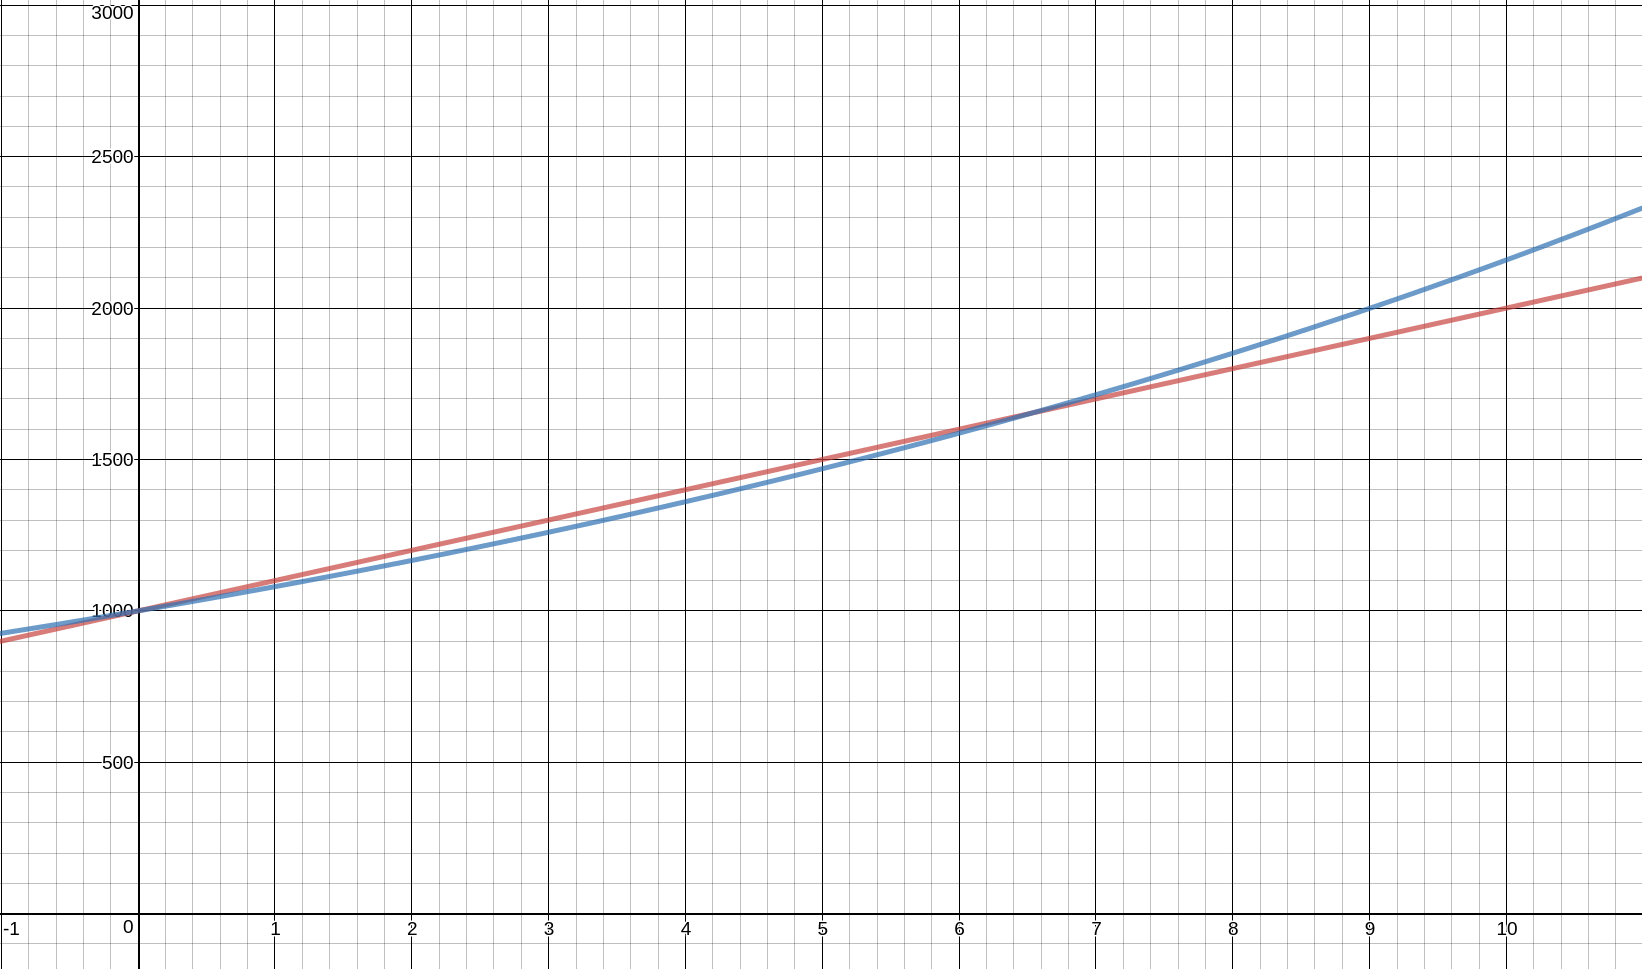
\includegraphics[width=0.9\textwidth]{img/interest_1.png}
 % interest_1.png: 0x0 pixel, 300dpi, 0.00x0.00 cm, bb=
\end{center}

Graph generated and viewable at \url{https://www.desmos.com/calculator/ablq5wdunm} 
 
\end{frame}



\begin{frame}
 \frametitle {  Which bank would you use?   }
 How big would the difference be after 20 years? 
 \only<2>{
 \begin{center}
 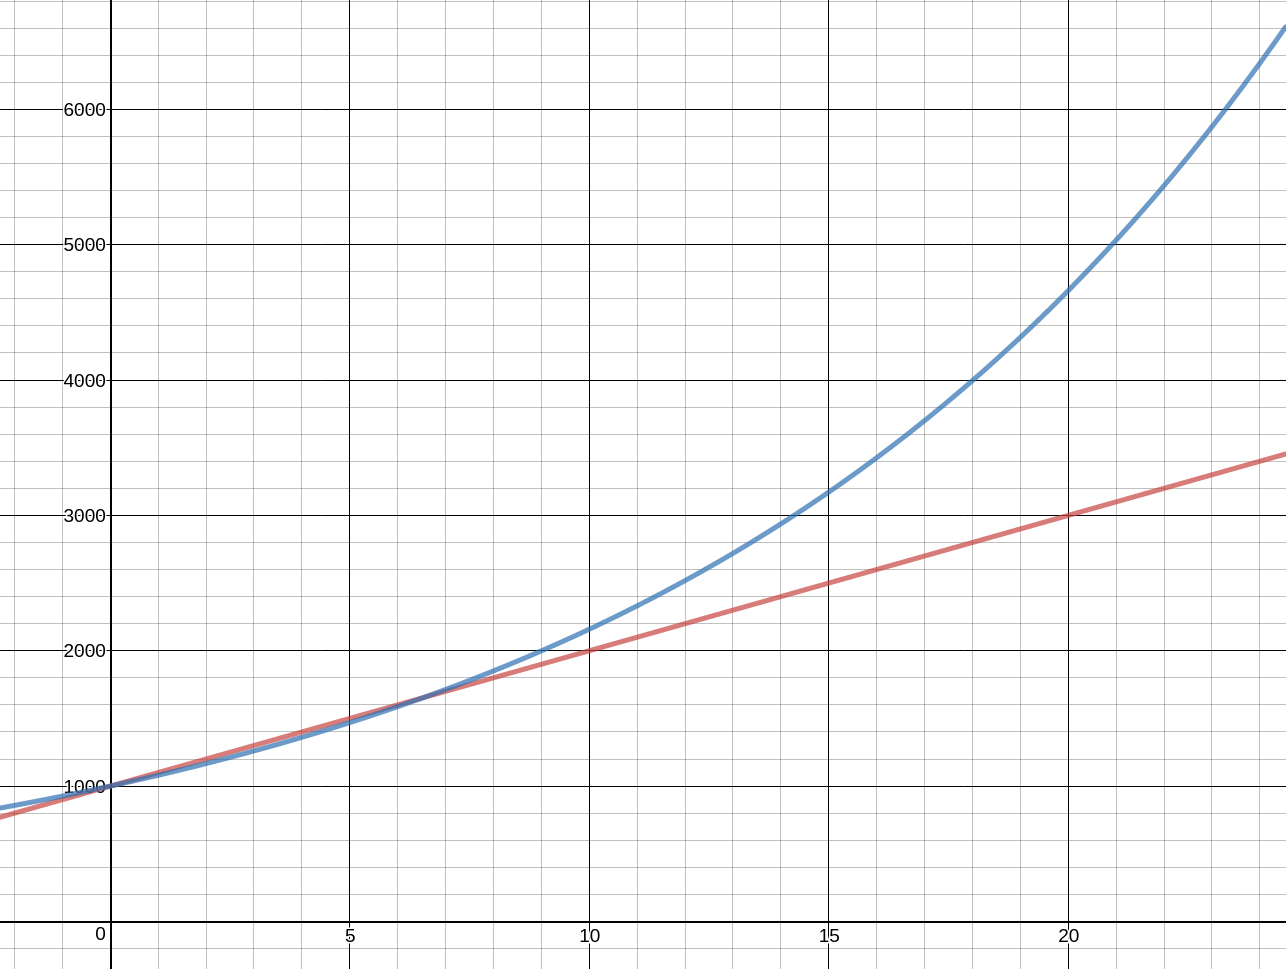
\includegraphics[width=0.8\textwidth]{img/interest_2.png}
 % interest_1.png: 0x0 pixel, 300dpi, 0.00x0.00 cm, bb=
\end{center}
}

\end{frame}





% \begin{frame} 
%   
%   \begin{beamerboxesrounded}[upper=palette tertiary,lower=palette secondary,shadow=true]{Linear vs. Exponential Growth }
%      In linear growth, the absolute change in constant. 
%      
%      In exponential growth, the absolute change 
% 
%     
%   \end{beamerboxesrounded}
%  
% 
% \end{frame}


\section{Significance of Doubling}



\begin{frame}
 \frametitle { Rice and the Chessboard Story  } 
 

 \begin{itemize}[<*>] 
  \item The creator of the game of chess showed his invention to the ruler, the ruler was highly impressed. 
 
  \item He was so impressed, in fact,  that he told the inventor to name a prize of his choice. 
 
  \item The inventor, being rather clever, said he would take a grain of rice on the first square of the chessboard, two grains of 
 rice on the second square of the chessboard, four on the third square, eight on the fourth square, and so on, doubling the 
 number of grains of rice for each successive square. 
 
  \item The ruler laughed at such a modest prize, but he ordered his treasurer to count out the rice.
 
 \end{itemize}
% %  \only<5->{The treasurer took more than a week to count the rice in the ruler’s store, only to notify the ruler that it would take more 
% %  rice than was available in the entire kingdom. }
% %  
% %  \only<6->{(Shortly thereafter, as the story goes, the inventor became the new king.)}

 

\end{frame}




\begin{frame}
 \frametitle{ Rice and the Chessboard Story  } 
 
 \begin{itemize}
  \item What do you think about the prize that the creator of chess asked for? 
  \item Can you guess how many grains of rice will he receive? 
 \end{itemize}


\end{frame}




\begin{frame}
 \frametitle { Rice and the Chessboard Story  } 
 

 \begin{itemize}[<*>] 
   \item ... 
  \item The treasurer took more than a week to count the rice in the ruler’s store, only to notify the ruler that it would take more 
 rice than was available in the entire kingdom. 
 
  \item (Shortly thereafter, as the story goes, the inventor became the new king.)

 \end{itemize}
 

\end{frame}



\begin{frame}
 \frametitle {  Rice and the Chessboard Story    }
 How many grains? 
 
 \begin{itemize} [<*>] 
  \item square 1: 1 grain
  \item square 2: 2 grains 
  \item square 3: 4 grains 
  \item square 4: 8 grains 
  \item square 5: 16 grains 
  \item square 6: 32 grains 
  \item square 7: 64 grains 
 \end{itemize}
 
 Can you see the pattern? What would the number of grains be for a square $s$?
 
 \only<2->{
  
  \center{square $s$ : $2^{s-1}$ grains }
 
 }

\end{frame}


\begin{frame}
 \frametitle {  Rice and the Chessboard Story    }
 How big is $2^{s-1}$ ? 
 
 \begin{itemize} [<*>] 
  \item square 5: so $s=5$ and  $2^{5-1} = 16$ grains   
  \item ... 
  \item square 10: so $s=10$ and  $2^{10-1} = 512$ grains   
  \item ... 
  \item square 16: so $s=16$ and  $2^{16-1} = 32,768 $ grains  
  \item ... 
  \item square 32: so $s=16$ and  $2^{32-1} = 2,147,483,648 $ grains   
  \item ... 
  \item square 64: so $s=16$ and  $2^{32-1} = 9,223,372,036,854,775,808 $ grains   
 \end{itemize}
 

 
 \only<2->{ \small 
    According to some source the white long grain rice yields ~29,000 grains in 1 pound of rice. 
    This gives us ~ 318,047,311,615,682 pounds, or 159,023,655,807 tons of rice just for the last square of the chessboard. 
  }
 

\end{frame}


\section{Population Growth} 



\begin{frame}
 \frametitle {   }
 \begin{center}
 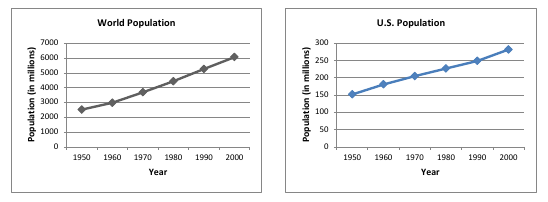
\includegraphics[width=1\textwidth]{img/population_growth.png}
 % population_growth.png: 0x0 pixel, 300dpi, 0.00x0.00 cm, bb=
\end{center}

\small{
Two students, Jane and Jack, are looking at the above graphs for their political science 
class report.

\textbf{Jane:}  It looks like the U.S. population grew the same amount as the world population, but that can’t be right, can it?

\textbf{Jack:}  Well, I don’t think they grew by the same amount, but they sure grew at about the same rate. Look at the slopes.
}
 

\end{frame}





\begin{frame}
 \frametitle {  World vs. U.S. Population  } 
 
 Work with a partner to try to answer the following questions: 
 \scriptsize{ 
 \begin{itemize} [<*>]
  \item Is Jane's observation correct? Why or why not?
  \item Is Jack's observation correct? Why or why not? 
  \item Estimate the percent increase in world population from 1950 to 2000.
  \item Estimate the percent increase in U.S. population from 1950 to 2000.
  \item How do those two compare? 
  \item Do the graphs above seem to indicate linear or exponential population growth? Explain your response. 
  \item Write an explicit formula for the sequene that models the world population growth from 1950 to 2000 based
  on the information in the graph. Assume the population (in millions) in 1950 was 2,500 and in 2000 was 6,000. Use $t$ to
  represent the number of years after 1950. 
  \item Test the above formula by calculating the size of world population in 2000. Do you get an answer consistent with the graph?
  If not, you should revise the formula. 
  \item Write a formula for U.S. population. Assume the population (in millions) in 1950 was 150 and in 2000 was 280. Use $t$ to
  represent the number of years after 1950. 
  \item Test the above formula by calculating the size of world population in 2000. Do you get an answer consistent with the graph?
  If not, you should revise the formula. 
  \item Use the last formula to calculate the U.S. population in 2010. Use google to check the actual population. Are the two values
  consistent? 
  
 \end{itemize}
}

\end{frame}



\begin{frame}
 \frametitle { A sweet old lady ... }
 
 
 \begin{itemize}
  \item  \textit{I met a sweet old lady yesterday when I was waiting for the train.
  We started talking and she told me about her four adult children and their wonderful life and
  how very proud she was of her seventeen grandchildren ...} 
  \item \textit{ All I was thinking: "Oh my gosh! This is exponential growth!" }
  \vspace{1em}
  \item Is it really exponential growth? Why?
  \item Assuming the same type of growth for the next generation, how many great-grandchildren
  will the \textit{sweet old lady} have? 
  \item Assuming the same type of growth for the following generation, how many
  great-great-grandchildren will she have? 
        
 \end{itemize}

\end{frame}




\begin{frame}
 \frametitle {Human generation   } 
 
 \begin{itemize}
  \item How many years is one human generation?
   \begin{itemize}
    \item This will vary from one culture to another, from one part of the country to another
    and from one family to another. 
    \item Right now, most estimates claim that it is \texttildelow25 years 
    \item See \url{http://isogg.org/wiki/How_long_is_a_generation\%3F_Science_provides_an_answer}
    for more scientific discussion 
   \end{itemize}
  \item The first Dutch settled (made land claims) in the New York area in 1609. How many generations 
  is it since then? 
  \begin{itemize}
   \item Assuming \texttildelow25 years per generation, there are 4 generations in each century (100 years). 
   \item In \texttildelow400 years, we have 16 generations. 
  \end{itemize}
  \item The ancient Egypt dates back to \texttildelow3100 B.C. How many generations is it since then? 
  \begin{itemize}
   \item It is the same 4 generations per century.
   \item Now we have \texttildelow50 centuries, so it is approximately 200 generations. 
  \end{itemize}

 \end{itemize}

\end{frame}



\begin{frame}
 \frametitle {  Human generations and population growth  }
 
 \hfill 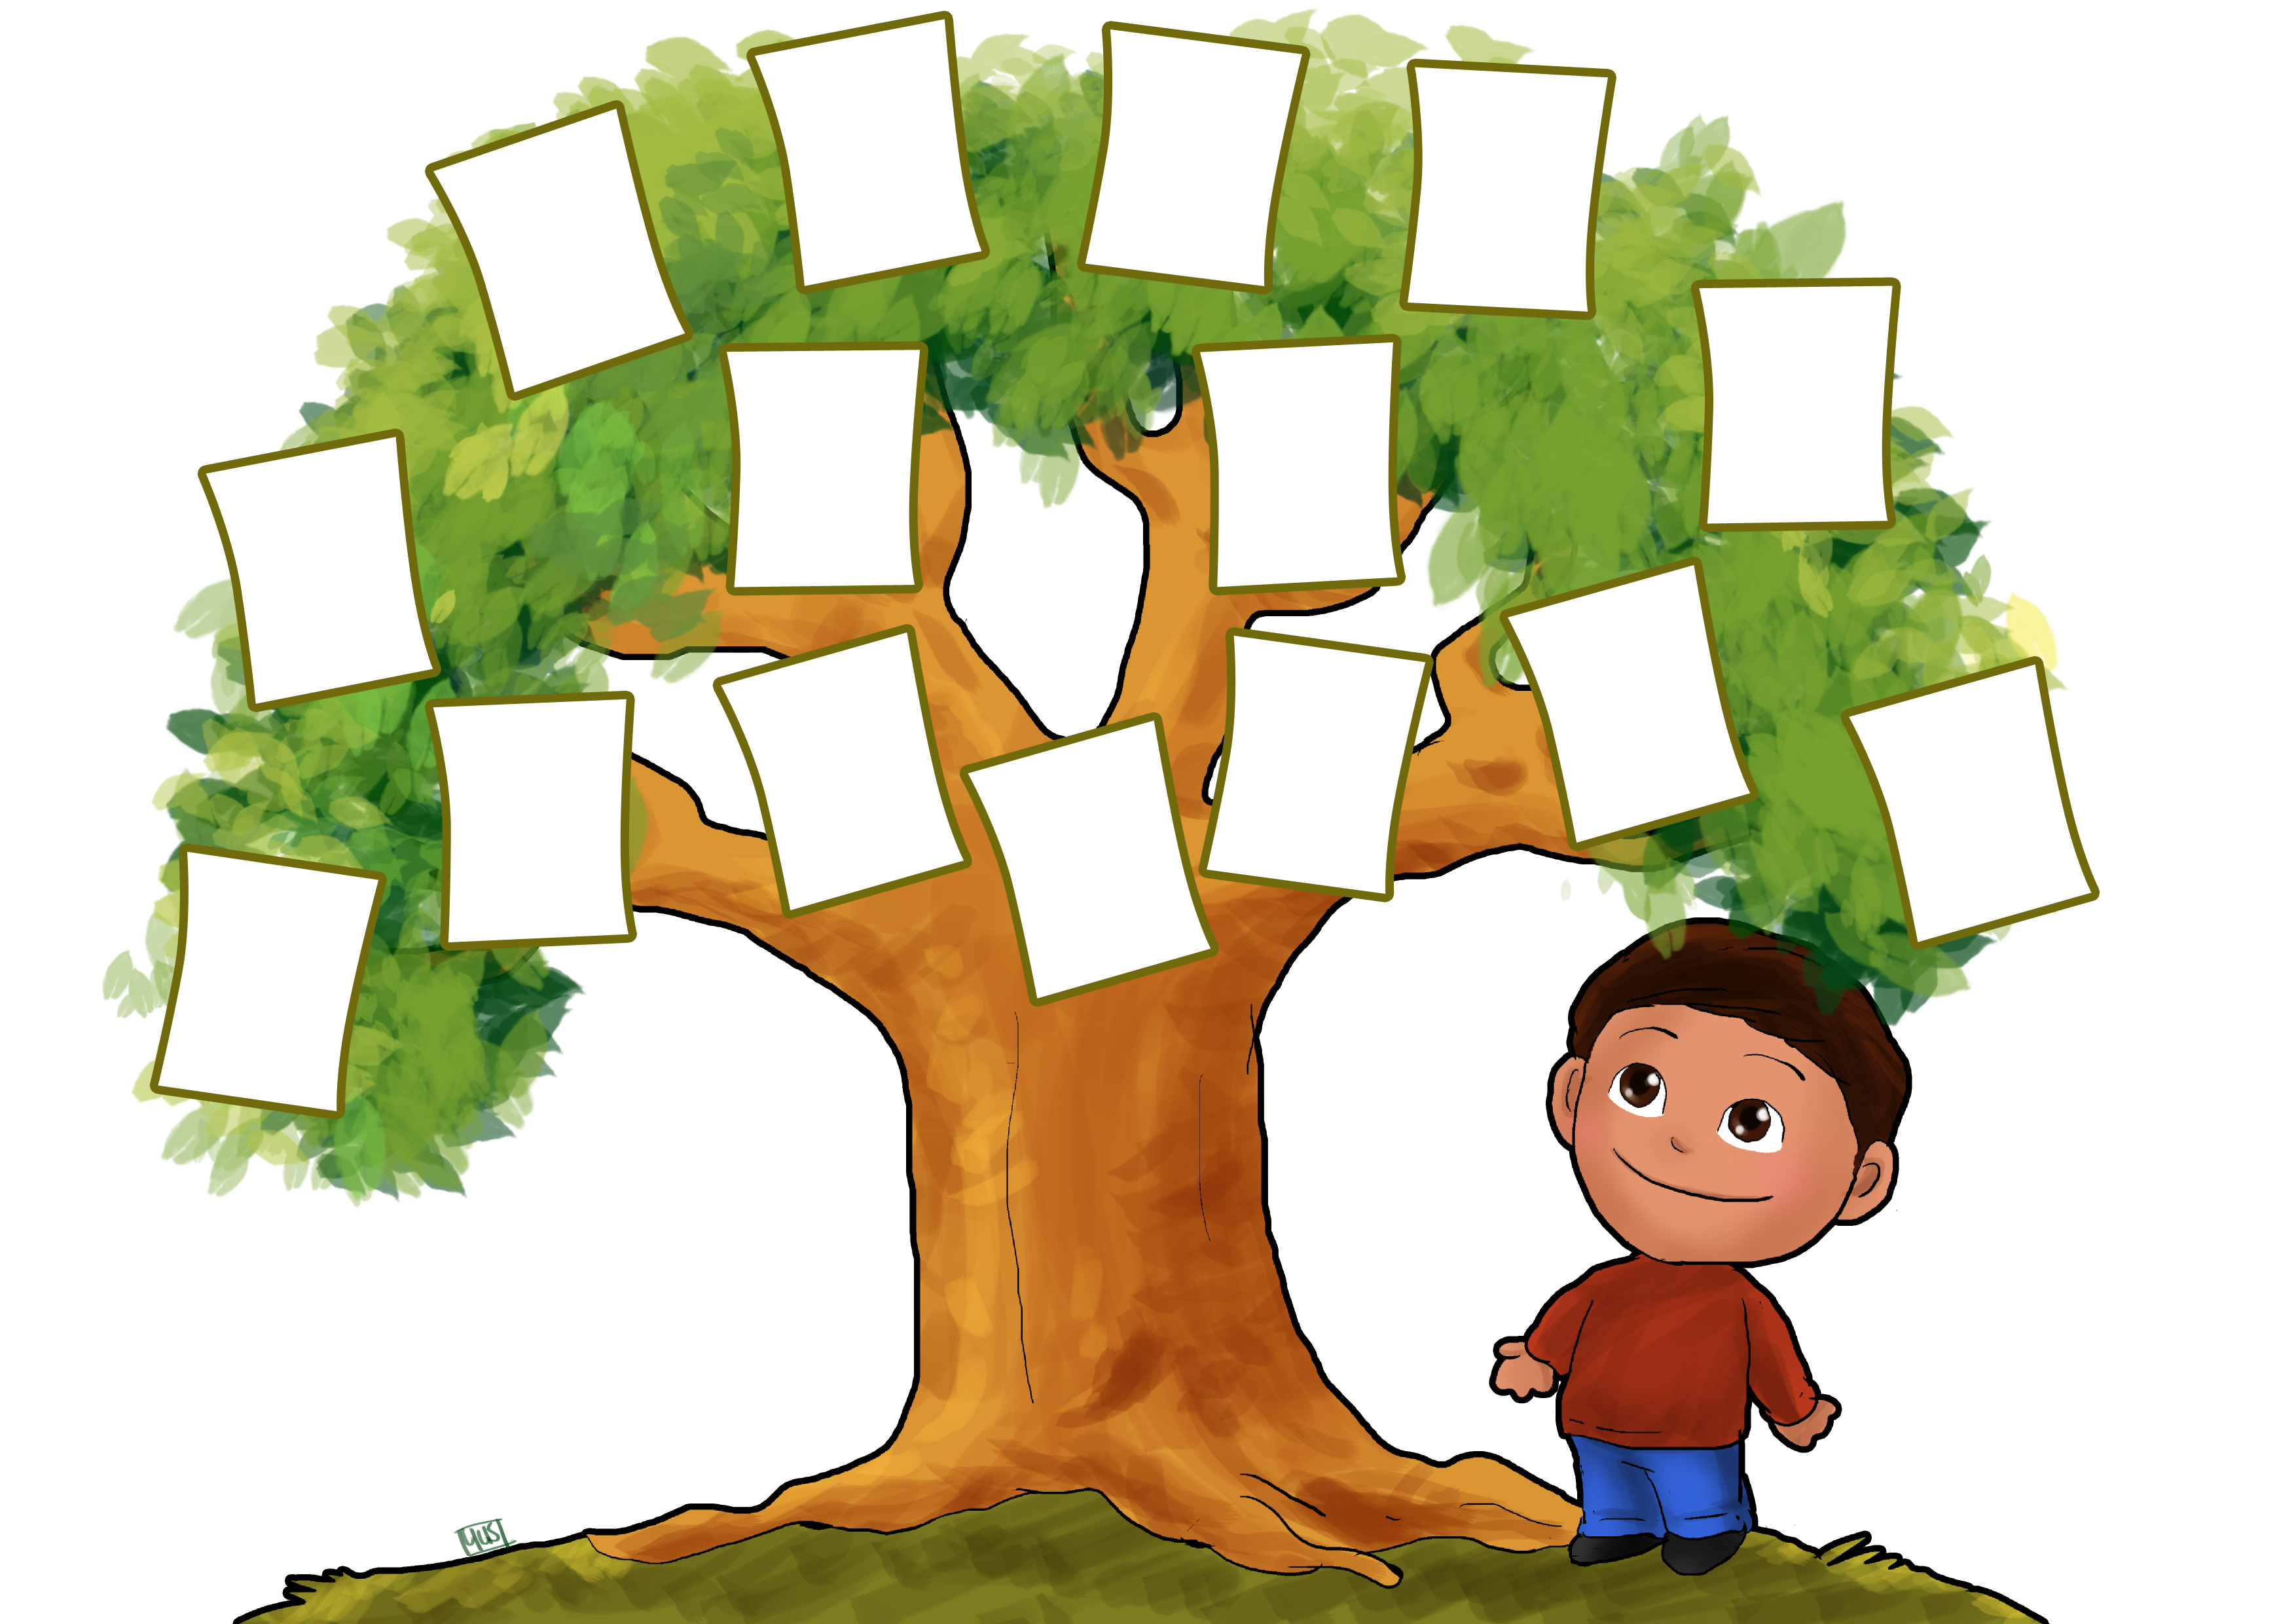
\includegraphics[width=0.3\textwidth]{img/family-tree.jpg}
% family-tree.jpg: 0x0 pixel, 300dpi, 0.00x0.00 cm, bb=


 
 \begin{itemize}
  \item Assume that each generation in a family line produces 2 offsprings. 
  \item Consider your ancestor from 4 generations ago (your great-grandmother), how many "relatives" do you 
  have from that branch of a family tree? 
  \begin{itemize}
   \item 1 - great-grandmother
   \item 2 - grandparent 
   \item 4 - parent 
   \item 16 - you 
   
  \end{itemize}

 \end{itemize}

\end{frame}


\begin{frame}
 \frametitle {  Human generations and population growth  }
 
 \begin{itemize}
  \item What if each generation produced 3 offsprings, how many "relatives" do you 
  have from that branch of a family tree in four generations? 
  \item \footnotesize{
  \begin{itemize}[<*>]
   \item 1 - great-grandmother
   \item 3 - grandparent 
   \item 9 - parent 
   \item 27 - you 
   
  \end{itemize}
  }
  \vspace{1em} 
  \item What if each generation produced 6 offsprings, how many "relatives" do you 
  have from that branch of a family tree in four generations? 
  \item \footnotesize{
  \begin{itemize}[<*>]
   \item 1 - great-grandmother
   \item 6 - grandparent 
   \item 36 - parent 
   \item 216 - you 
  \end{itemize}
  } 
  \vspace{1em}  
  \item What is the function that we can use to calculate this? 
  \begin{itemize}
   \item $r(g) = n^g$ 
   \item $g$ is the number of generations, $n$ is the number of offsprings per generation, $r(g)$ is the function of number of
   generation that calculates the number of "relatives" 
  \end{itemize}

  

 \end{itemize}

\end{frame}



\begin{frame}
 \frametitle { Other Factors of Human Population    }
 
 Birth rates (i.e., the number of offsprings per generation) are not the only factors 
 that influence the current size of human population.
 \vspace{2em}
 
 What are some other factors? 


\end{frame}








\begin{frame}
\center{ 
 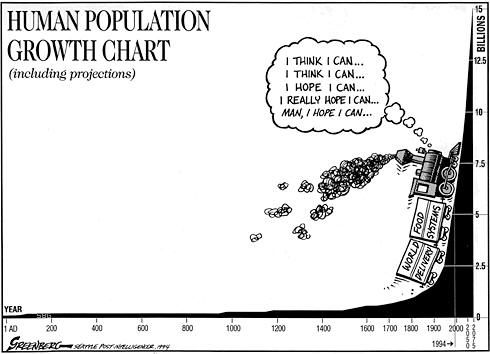
\includegraphics[width=0.99\textwidth ]{img/population_growth.jpg}
% population_growth.jpg: 0x0 pixel, 300dpi, 0.00x0.00 cm, bb=
 }
\end{frame}


\section{Borrowing and Saving} 



\begin{frame}
 \frametitle { Credit Cards  }
 
 \begin{itemize} [<*>]
  \item John Doe charged \$125.24 to his credit card during the last statement period. 
  \item His minimum payment due is \$20.00. 
  \item He decides to settle his debt with the credit card company by making the \$20.00
  monthly payments. \\
  He also is not going to be using this credit card anymore.
  \item The credit card company charges 1.65\% montly interest rate on the unpaid amount. 
  \item How many months will it take him to be debt free? \\
  How much extra is he going to pay the bank? 
 \end{itemize}

\end{frame}





\begin{frame}
 \begin{center}
    
  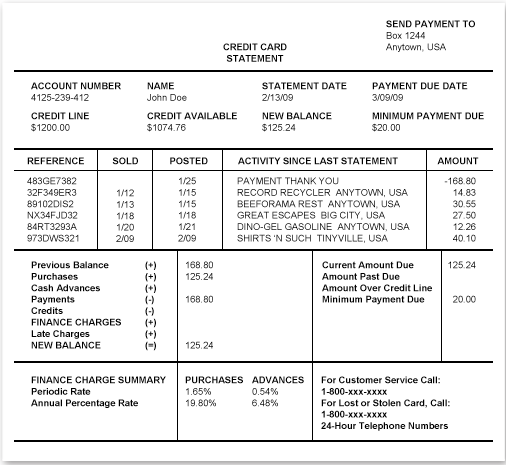
\includegraphics[height=0.8\textheight ]{img/credit_card.png}
  % population_growth.jpg: 0x0 pixel, 300dpi, 0.00x0.00 cm, bb=
 \end{center}

 
 \footnotesize{
 See \url{http://www.practicalmoneyskills.com/flash/bank_tutor/index.html} for 
 detailed explanation of parts of the above bill. 
}
\end{frame}




\begin{frame}
 \frametitle {  Credit Cards  }
  \footnotesize{ 
 \begin{itemize}
  \item month 0  (end of the current billing statement): 
  statement balance is \$125.24\\
  he pays \$20.00, balance is \$105.24 
  \item month 1:
   balance with interest is \$105.24 * (1 + 0.0165) = \$106.98, \\
   he pays \$20.00, remaining balance is \$86.98 
  \item month 2:
   balance with interest is \$86.98 * (1 + 0.0165) = \$88.41, \\
   he pays \$20.00, remaining balance is \$68.41 
  \item month 3: 
   balance with interest is \$68.41 * (1 + 0.0165) = \$69.54, \\
   he pays \$20.00, remaining balance is \$49.54 
  \item month 4: 
   balance with interest is \$49.54  * (1 + 0.0165) = \$50.36, \\
   he pays \$20.00, remaining balance is \$30.36 
  \item month 5: 
   balance with interest is \$30.36  * (1 + 0.0165) = \$30.86, \\
   he pays \$20.00, remaining balance is \$10.86 
  \item month 6:
   balance with interest is \$10.86  * (1 + 0.0165) = \$11.04, \\
   he pays the remaining balance \$11.04
   
  \vspace{1em}
  \item There is a total of \$5.81 interest paid over those six months. Does not seem like much, does it?
  \item What is the annual interest rate that this credit card charges? 
 \end{itemize}
  }


\end{frame}





\begin{frame}
 \frametitle {   Credit Cards   }
 
 \begin{itemize}
  \item Think about:
  \begin{itemize}
   \item How is the value of interest paid affected by the interest rate?
   \item How is the value of interest paid affected by the initial balance?
   \item How is the value of interest paid affected by the amount of monthly payments? 
   \vspace{2em}
   \item What is the function that calculates the total amount that will be paid
   with the fixed monthly payments and fixed interest rate? 
   \item What is the function that calculated the payment balance after each month 
   with the fixed monthly payments and fixed interest rate? 
  \end{itemize}

 \end{itemize}


\end{frame}





\begin{frame}
 \frametitle { Saving For Retirement   } 
 
 Simplified model:
 
 \begin{itemize}
  \item At the end of each year (till your retirement) you deposit \$1000.00 in 
  your retirement account. 
  \item The brokerage managing your money, guarantees that they can make 5\% interest
  on the balance of the account each year. 
  \item How much money will there be in the account in 1 year, 2 year, 10 year, 20 years? 
  \begin{itemize}
   \item year 0: deposit \$1000.00, no interest yet 
   \item year 1: balance plus interest \$1000.00 ( 1 + 0.05) = \$1050.00 \\
   new deposit:  \$1000.00, total: \$2050.00 
   \item year 2: balance plus interest \$2050.00 ( 1 + 0.05) = \$2152.50 \\ 
   new deposit:  \$1000.00, total:  \$3152.50 
   \item ...
  \end{itemize}

 \end{itemize}


\end{frame}




\begin{frame}
 \begin{center}
    
  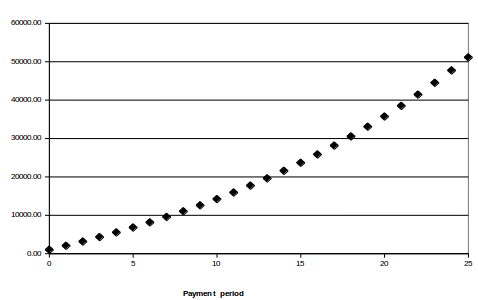
\includegraphics[height=0.8\textheight ]{img/retirement_1.png}
  % population_growth.jpg: 0x0 pixel, 300dpi, 0.00x0.00 cm, bb=
 \end{center}

 
 \footnotesize{
 After 25 years of this pattern, the balance on the account is \$51,113.45. 
}
\end{frame}






\section{Exercises} 







\begin{frame}
 \frametitle{ Try it Yourself  }
 
\scriptsize{  
 \textbf{ NY State Population Growth: } 
 
 The table below represents the population of the state of New York for the years 1800–2000. Use this information
to answer the questions.

\begin{center}
\begin{tabular}{cc}
Year & Population\\
1800 & 300,000\\
1900 & 7,300,000\\
2000 & 19,000,000
\end{tabular}
\end{center}

\begin{itemize}  [<*>] 
 \item Using the year 1800 as the base year, an explicit formula for the sequence that models the population of New
York is P(t) = 300 000(1.021)t , where t is the number of years after 1800.

Using this formula, calculate the projected population of New York in 2010.

 \item 
Using the year 1900 as the base year, an explicit formula for the sequence that models the population of New
York is P(t) = 7 300 000(1.0096)t, where t is the number of years after 1900.

Using this formula, calculate the projected population of New York in 2010.


 \item Using the Internet (or some other source), find the population of the state of New York according to the 2010
census. Which formula yielded a more accurate prediction of the 2010 population?

 \item (Extra Challenge) Figure out how the formulas in the above questions were derived. 
\end{itemize}

}
 
\end{frame}



\begin{frame}
 \frametitle { Try it Yourself  }
 
 \begin{itemize} [<*>]
 
  \item A rare coin appreciates at a rate of 5.2\% a year. If the initial value of the coin is \$500, after how many years will its
value cross the \$3,000 mark? Show the formula that models the value of the coin after t years.
 
  \item A local college has increased its number of graduates by a factor of 1.045 over the previous year for every year since
1999. In 1999, 924 students graduated. What explicit formula models this situation? Approximately how many
students will graduate in 2014?
 
 
 \item A three-bedroom house in Burbville sold for \$190,000. If housing prices are expected to increase 1.8\% annually in
that town, write an explicit formula that models the price of the house in t years. Find the price of the house in 5
years. 

 
 \end{itemize}
\end{frame}
% 
% 

\begin{frame}
 \frametitle { Try It Yourself  }
 Retirement savings
 \begin{itemize} [<*>] 
  \item What is the function that would calculate the value of your retirement
  assuming a fixed interest rate and fixed yearly deposit? 
  \item How does this formula compare to the credit card payment formula?
  \item How would the value of your retirement account change if the payments were
  made monthly and interest compounded monthly?
  \item How much would be in your retirement account if you were earning interest equal 
  to the interest rate charged by the banks on your credit card balance? 
 \end{itemize}


\end{frame}


\end{document}
